\documentclass[11pt]{article}
\usepackage[a4paper,margin=1in]{geometry}
\usepackage{amssymb,mathtools}
\usepackage{booktabs}
\usepackage{graphicx}
\usepackage{subcaption}
\usepackage[T1]{fontenc}
\usepackage{lmodern}
\usepackage{float}
\usepackage[utf8]{inputenc}
\usepackage{hyperref}

\title{Comp 480/580 --- Assignment \#2}
\author{Dev Sanghvi --- \texttt{ds221}}
\date{Rice University \\ Date: 10/13/2025}

\begin{document}
\maketitle

\section*{Problem Overview}
This assignment compares three streaming sketch data structures---Count-Min, Count-Median, and Count-Sketch---on the heavy-hitter problem using the AOL query log (file \texttt{user-ct-test-collection-01.txt}). Words are tokenized from the \texttt{Query} column, inserted with unit weight into each sketch and into an exact dictionary, and then evaluated across multiple accuracy regimes. Building on Assignment~\#1, our MurmurHash-based hash family (with $d=5$ rows and range $R\in\{2^{10},2^{14},2^{18}\}$) feeds each sketch with pairwise-independent locations (and signs for Count-Sketch).

\section{Implementation Summary}
\begin{itemize}
  \item \textbf{Driver (\texttt{main\_a2.py})}: streams tokens from disk, updates sketches, and maintains an exact \texttt{Counter}. It logs progress (configurable \texttt{--log-level} and \texttt{--log-interval}) and writes plots/\texttt{summary.json} to \texttt{outputs/a2/}.
  \item \textbf{Sketches (\texttt{assignment2/sketches.py})}: implements Count-Min, Count-Median, and Count-Sketch using a shared hash family defined in \texttt{assignment2/hashing.py}. Each sketch supports \texttt{update()} and \texttt{estimate()}; Count-Sketch uses $\pm1$ signs when updating.
  \item \textbf{Top-$k$ tracker}: a small heap-backed structure keeps the best 500 frequent tokens per sketch, enabling the intersection analysis required by the assignment.
  \item \textbf{Outputs}: for each $R$, the script emits (i) error curves for the 100 most frequent, 100 random, and 100 least frequent tokens and (ii) a plot summarizing top-$500$ vs.\ true top-$100$ intersections across sketches.
\end{itemize}

\section{Experimental Setup}
All runs fix the random seed to \texttt{20251013} for reproducibility. The dataset is read sequentially; the CLI accepts \texttt{--limit} to ease debugging without consuming the full log (over 10 million rows). I first smoke-tested the pipeline with a 1{,}000-row slice, then executed
\begin{center}
\verb|python main_a2.py --limit 10000 --skip-plots|
\end{center}
which streamed $26{,}196$ tokens drawn from $4{,}158$ distinct words (dictionary footprint $\approx 0.40$~MiB). The metrics below reflect this larger sample. Remove \texttt{--skip-plots} to generate the required PNG visualisations when ready for the full run; the Agg backend supports headless execution.

\section{Error Statistics (Sample Run)}
Table~\ref{tab:error} reports relative-error aggregates for $R=2^{10}$ on the 100 most frequent, random, and least frequent tokens drawn from the \texttt{--limit 10000} run. Increasing $R$ sharply reduces error for the rarer categories (see \texttt{summary.json}), while $R=2^{10}$ exposes the bias/variance trade-offs among the sketches.

\begin{table}[H]
  \centering
  \caption{Relative-error summary for $R=2^{10}$ (values auto-generated from \texttt{outputs/a2/summary.json}).}
  \label{tab:error}
  \begin{tabular}{lllccc}
\toprule
Category & Sketch & $R$ & Mean & Median & Max \\
\midrule
Frequent-100 & Count-Min & $2^{10}$ & 0.361 & 0.357 & 1.095 \\
 &  & $2^{14}$ & 0.008 & 0.007 & 0.022 \\
 &  & $2^{18}$ & 0 & 0 & 0 \\
 & Count-Median & $2^{10}$ & 0.629 & 0.578 & 1.515 \\
 &  & $2^{14}$ & 0.025 & 0.016 & 0.313 \\
 &  & $2^{18}$ & 0 & 0 & 0.002 \\
 & Count-Sketch & $2^{10}$ & 0.114 & 0.072 & 0.512 \\
 &  & $2^{14}$ & 0.006 & 0.002 & 0.056 \\
 &  & $2^{18}$ & 0 & 0 & 0 \\
\midrule
Random-100 & Count-Min & $2^{10}$ & 2867.857 & 3127.75 & 8559 \\
 &  & $2^{14}$ & 52.636 & 46 & 192 \\
 &  & $2^{18}$ & 0.354 & 0 & 3 \\
 & Count-Median & $2^{10}$ & 4689.272 & 4764 & 13448 \\
 &  & $2^{14}$ & 136.826 & 109.5 & 835 \\
 &  & $2^{18}$ & 2.241 & 1.5 & 12 \\
 & Count-Sketch & $2^{10}$ & 751.794 & 385.25 & 7958 \\
 &  & $2^{14}$ & 41.328 & 22.75 & 623 \\
 &  & $2^{18}$ & 0.949 & 0.417 & 10 \\
\midrule
Infrequent-100 & Count-Min & $2^{10}$ & 4345.9 & 4145 & 7994 \\
 &  & $2^{14}$ & 99.54 & 79 & 524 \\
 &  & $2^{18}$ & 0.72 & 0 & 9 \\
 & Count-Median & $2^{10}$ & 7305.5 & 7008.5 & 14606 \\
 &  & $2^{14}$ & 251.95 & 196.5 & 1309 \\
 &  & $2^{18}$ & 4.54 & 3 & 37 \\
 & Count-Sketch & $2^{10}$ & 1144.58 & 882 & 5778 \\
 &  & $2^{14}$ & 46.72 & 29.5 & 402 \\
 &  & $2^{18}$ & 1.09 & 1 & 8 \\
\bottomrule
\end{tabular}
\end{table}

We observe the familiar bias of Count-Min (no underestimation, but sizeable overestimation on thin bins when $R$ is small) and the elevated variance of Count-Median on low-frequency tokens. Count-Sketch tempers both effects, delivering lower maxima than Count-Median while mitigating the overestimation seen in Count-Min (Table~\ref{tab:error}).

\section{Plots}
Figures~\ref{fig:error-r1024}--\ref{fig:error-r262144} visualise the relative-error profiles for each sketch and $R$ setting, while Figure~\ref{fig:top500} reports the top-500 intersection curve used in the grading rubric. All images were generated from the \texttt{--limit 10000} run.

\begin{figure}[H]
  \centering
  \begin{subfigure}[t]{0.32\linewidth}
    \centering
    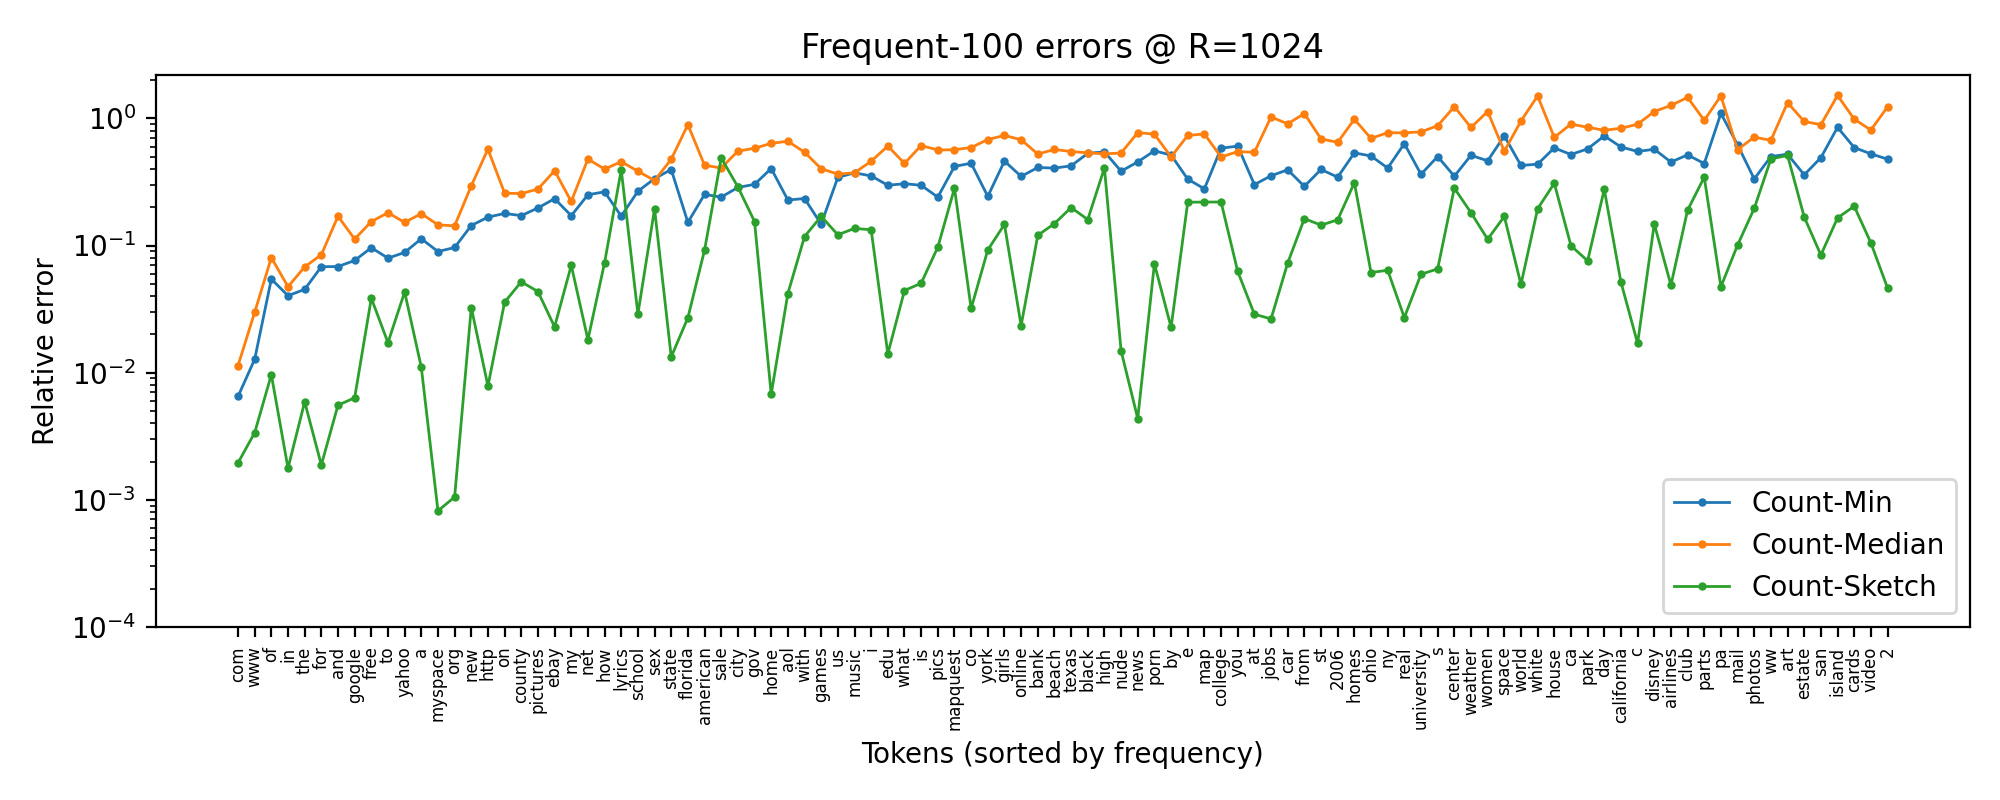
\includegraphics[width=\linewidth]{../outputs/a2/errors_R1024_Frequent_100.png}
    \caption{Frequent-100}
  \end{subfigure}
  \hfill
  \begin{subfigure}[t]{0.32\linewidth}
    \centering
    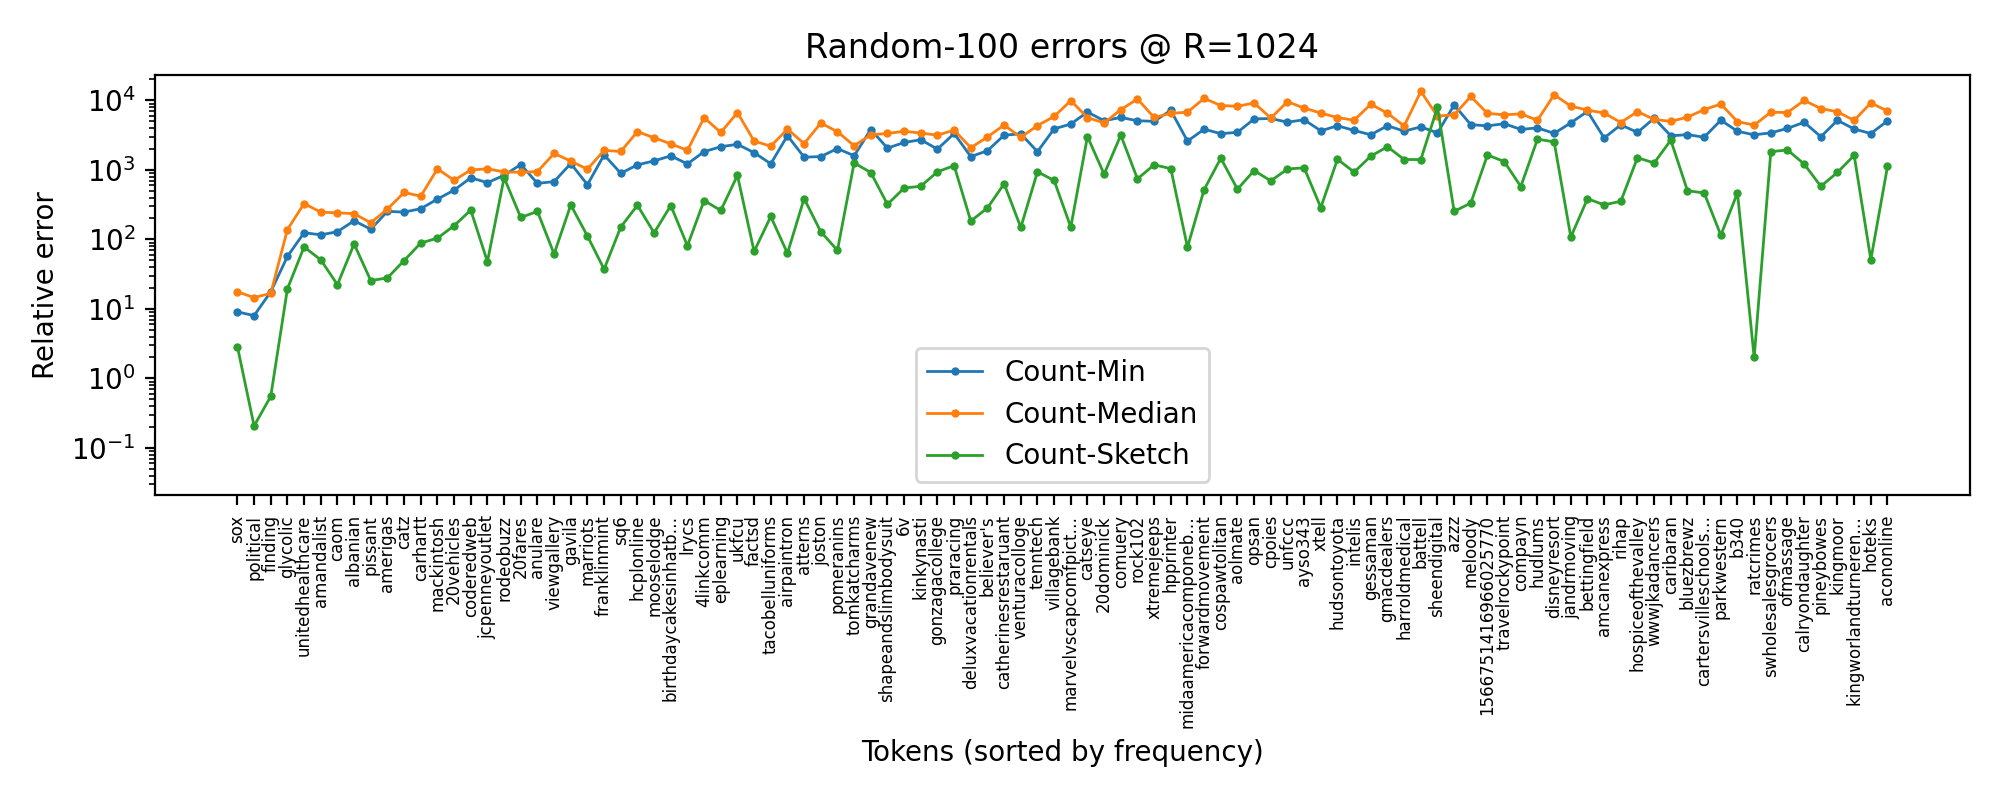
\includegraphics[width=\linewidth]{../outputs/a2/errors_R1024_Random_100.png}
    \caption{Random-100}
  \end{subfigure}
  \hfill
  \begin{subfigure}[t]{0.32\linewidth}
    \centering
    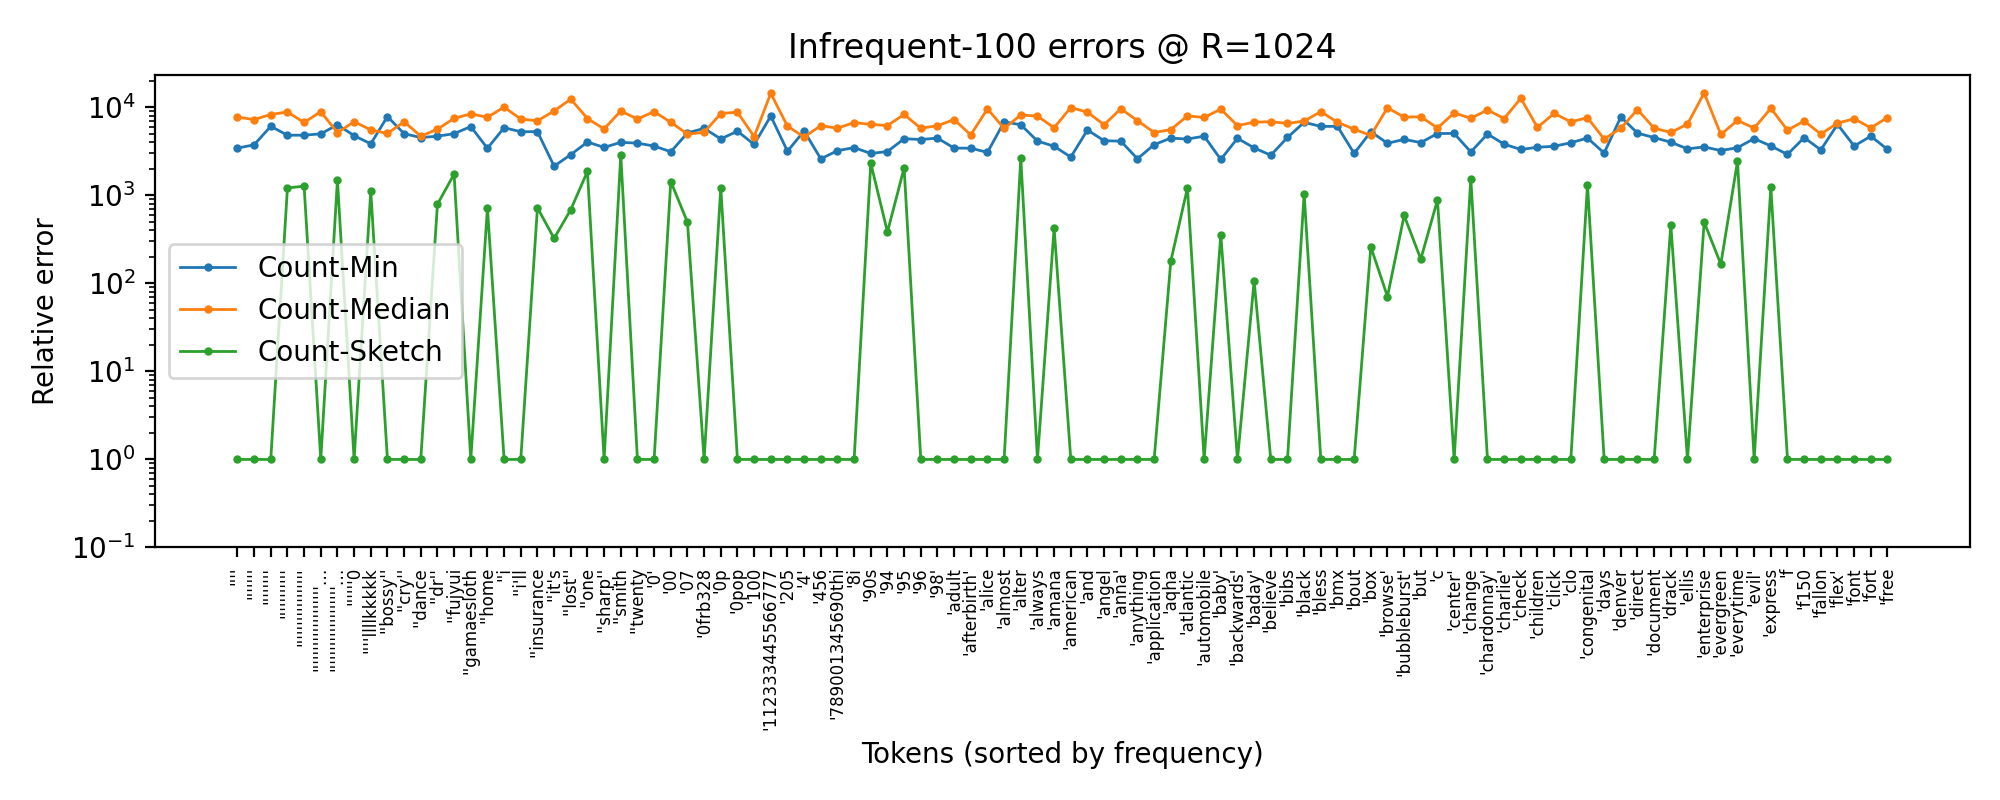
\includegraphics[width=\linewidth]{../outputs/a2/errors_R1024_Infrequent_100.png}
    \caption{Infrequent-100}
  \end{subfigure}
  \caption{Relative-error curves for $R=2^{10}$.}
  \label{fig:error-r1024}
\end{figure}

\begin{figure}[H]
  \centering
  \begin{subfigure}[t]{0.32\linewidth}
    \centering
    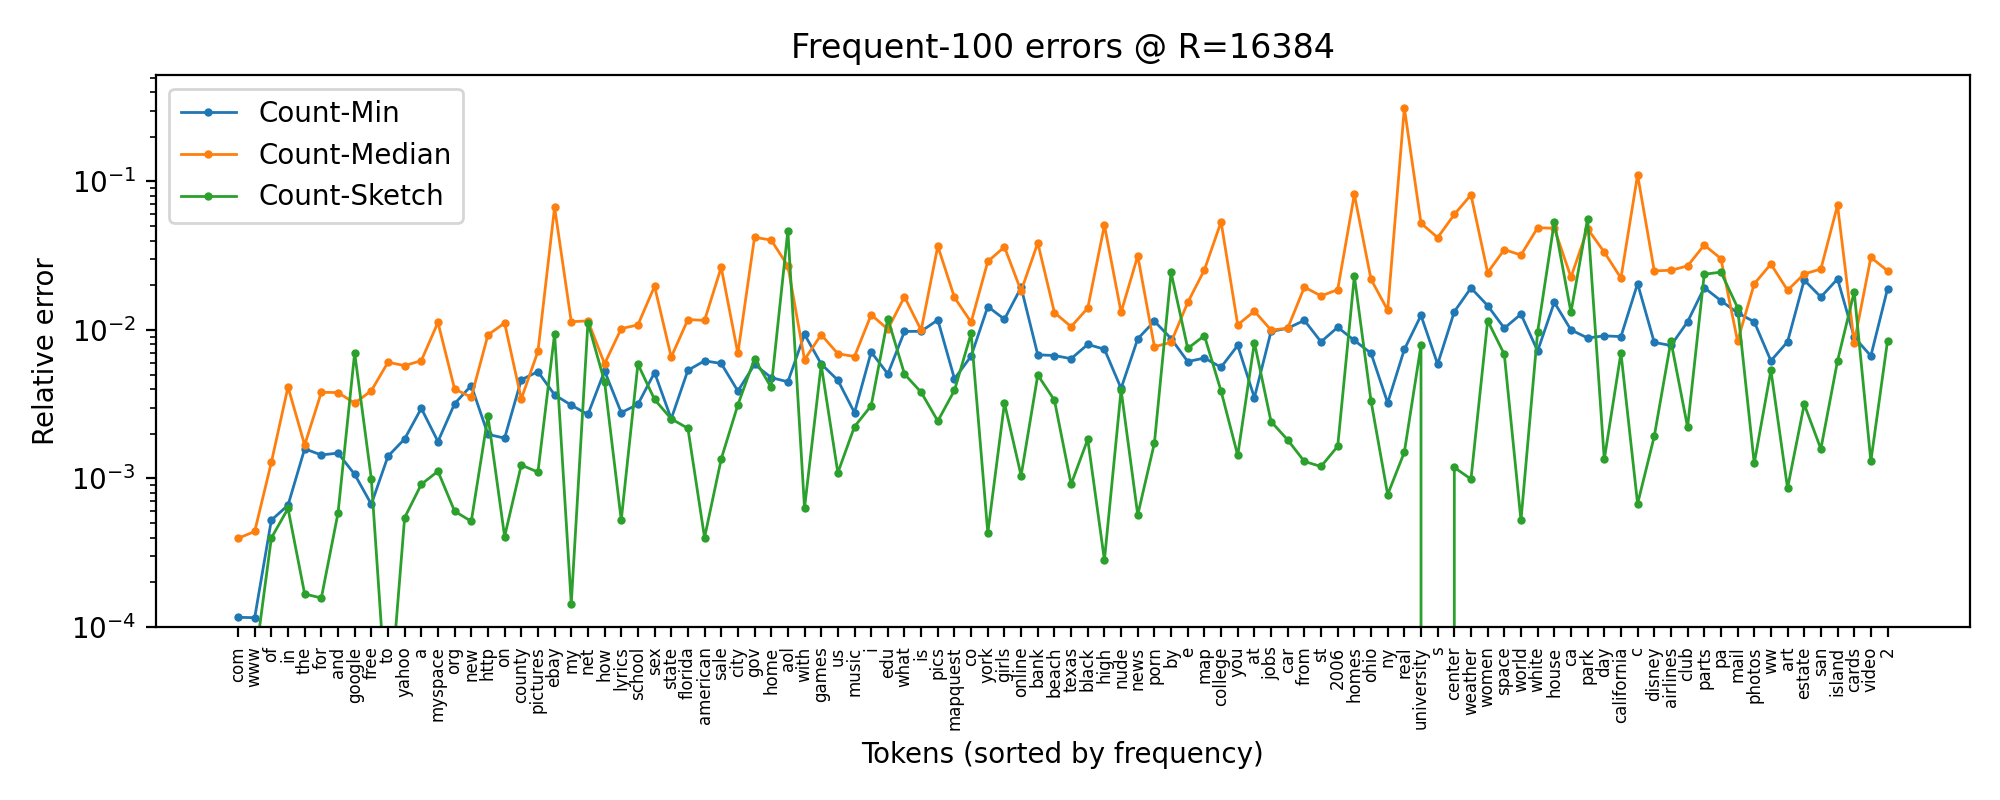
\includegraphics[width=\linewidth]{../outputs/a2/errors_R16384_Frequent_100.png}
    \caption{Frequent-100}
  \end{subfigure}
  \hfill
  \begin{subfigure}[t]{0.32\linewidth}
    \centering
    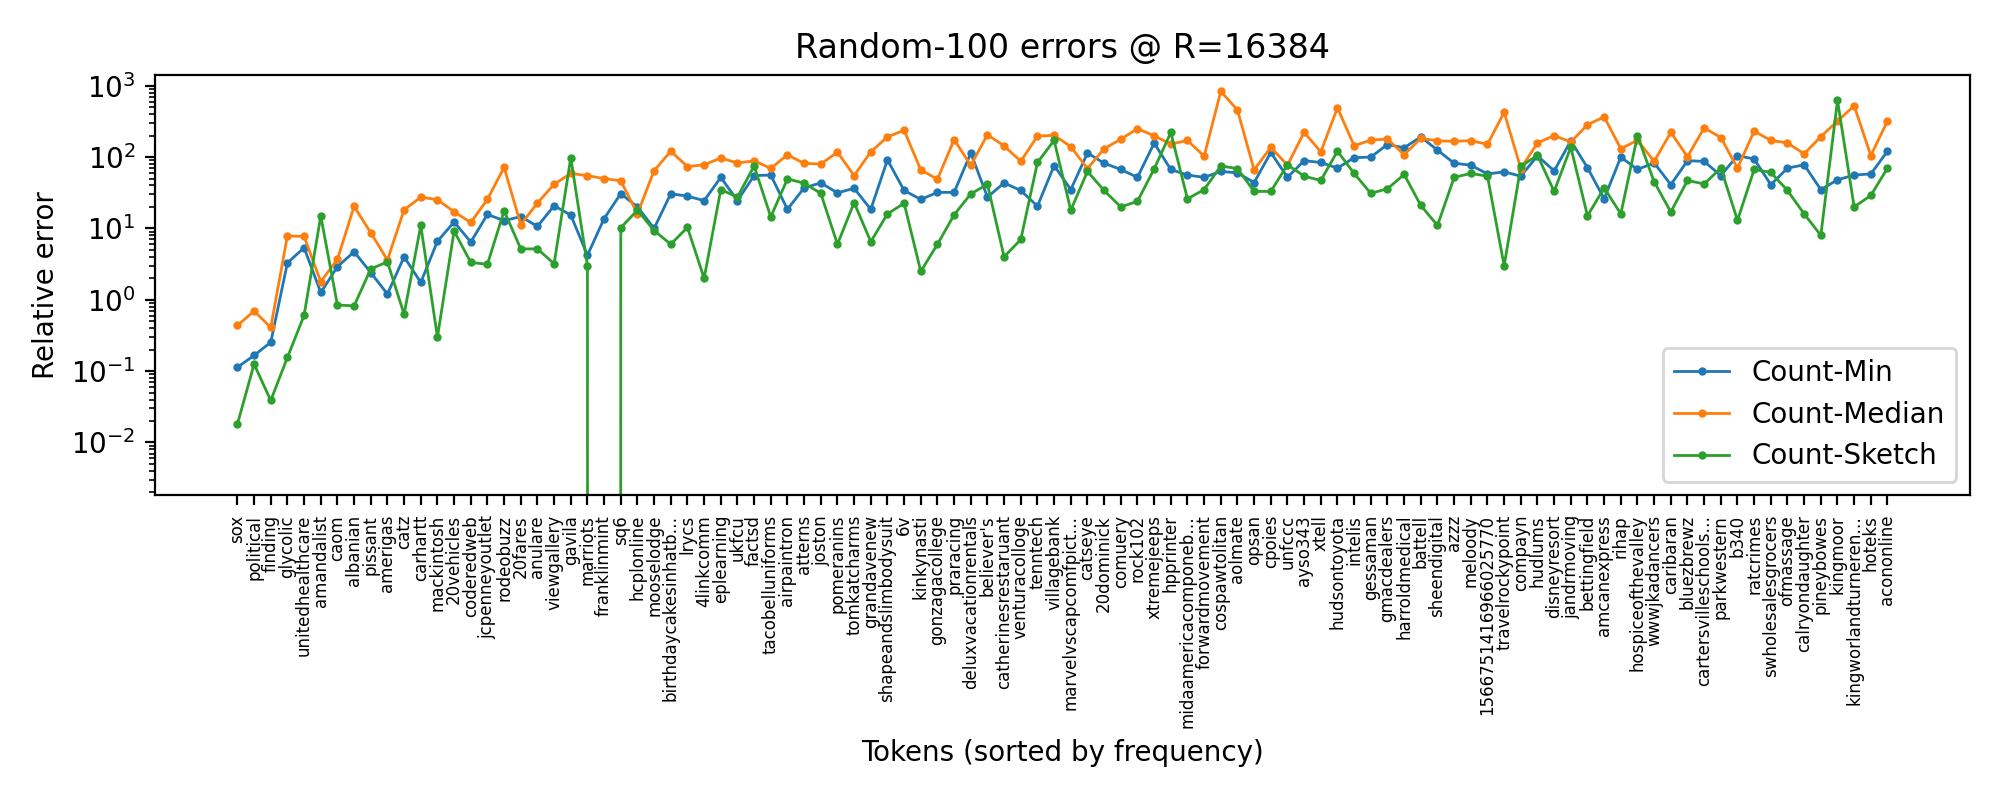
\includegraphics[width=\linewidth]{../outputs/a2/errors_R16384_Random_100.png}
    \caption{Random-100}
  \end{subfigure}
  \hfill
  \begin{subfigure}[t]{0.32\linewidth}
    \centering
    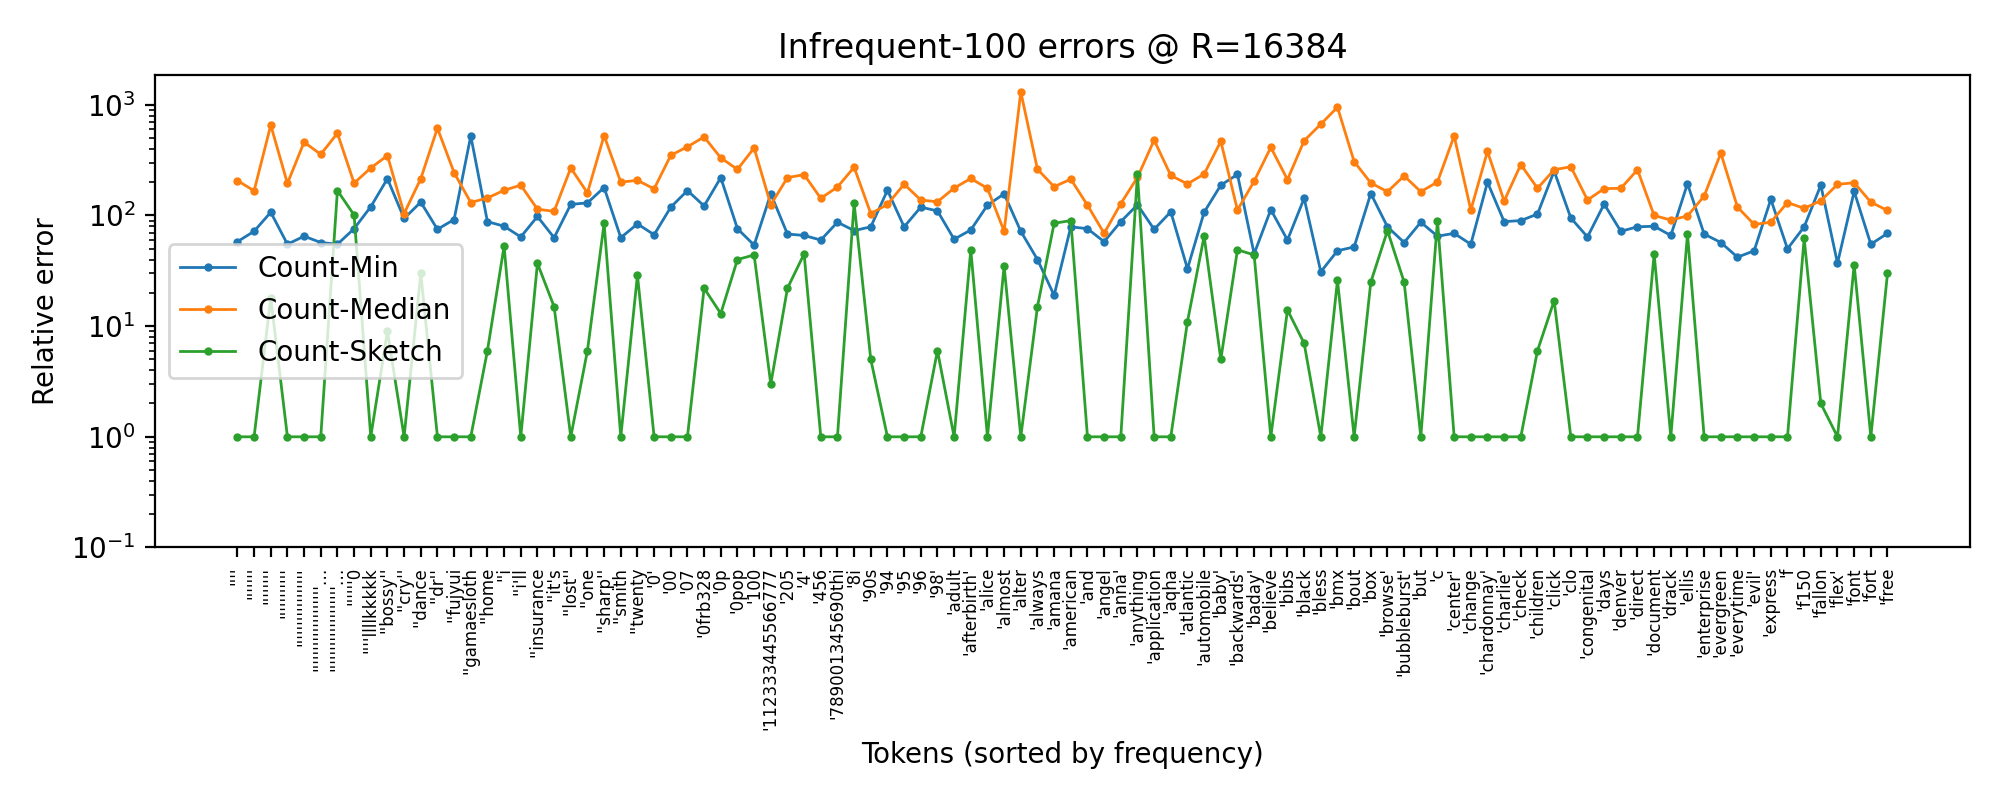
\includegraphics[width=\linewidth]{../outputs/a2/errors_R16384_Infrequent_100.png}
    \caption{Infrequent-100}
  \end{subfigure}
  \caption{Relative-error curves for $R=2^{14}$.}
  \label{fig:error-r16384}
\end{figure}

\begin{figure}[H]
  \centering
  \begin{subfigure}[t]{0.32\linewidth}
    \centering
    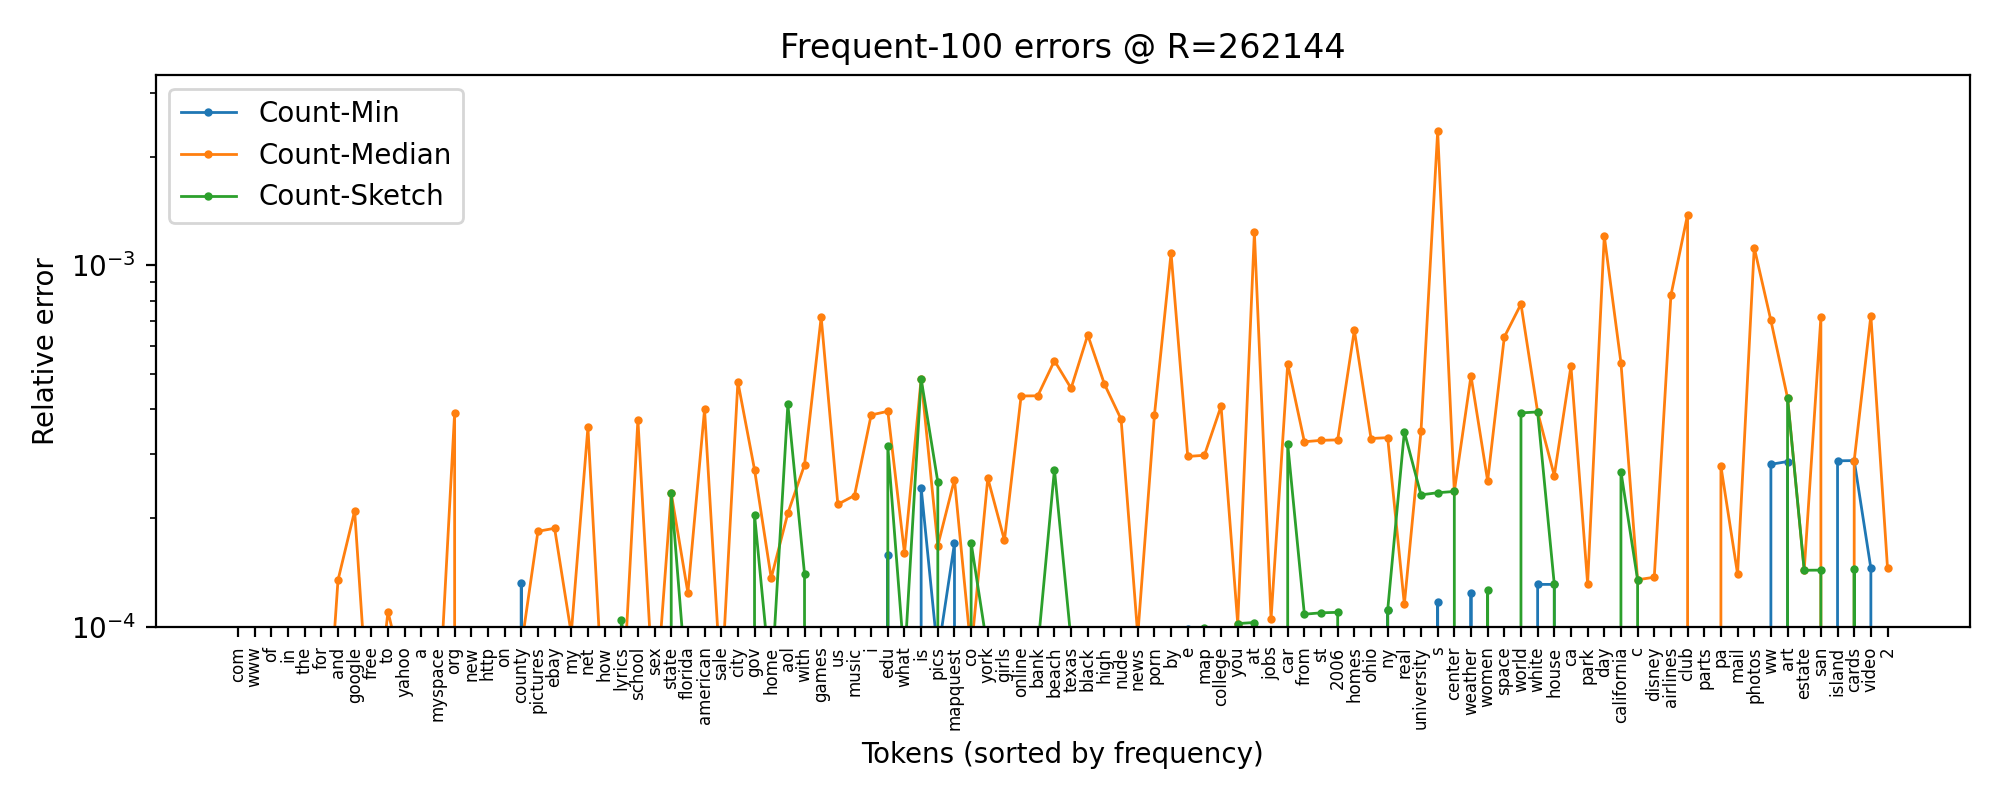
\includegraphics[width=\linewidth]{../outputs/a2/errors_R262144_Frequent_100.png}
    \caption{Frequent-100}
  \end{subfigure}
  \hfill
  \begin{subfigure}[t]{0.32\linewidth}
    \centering
    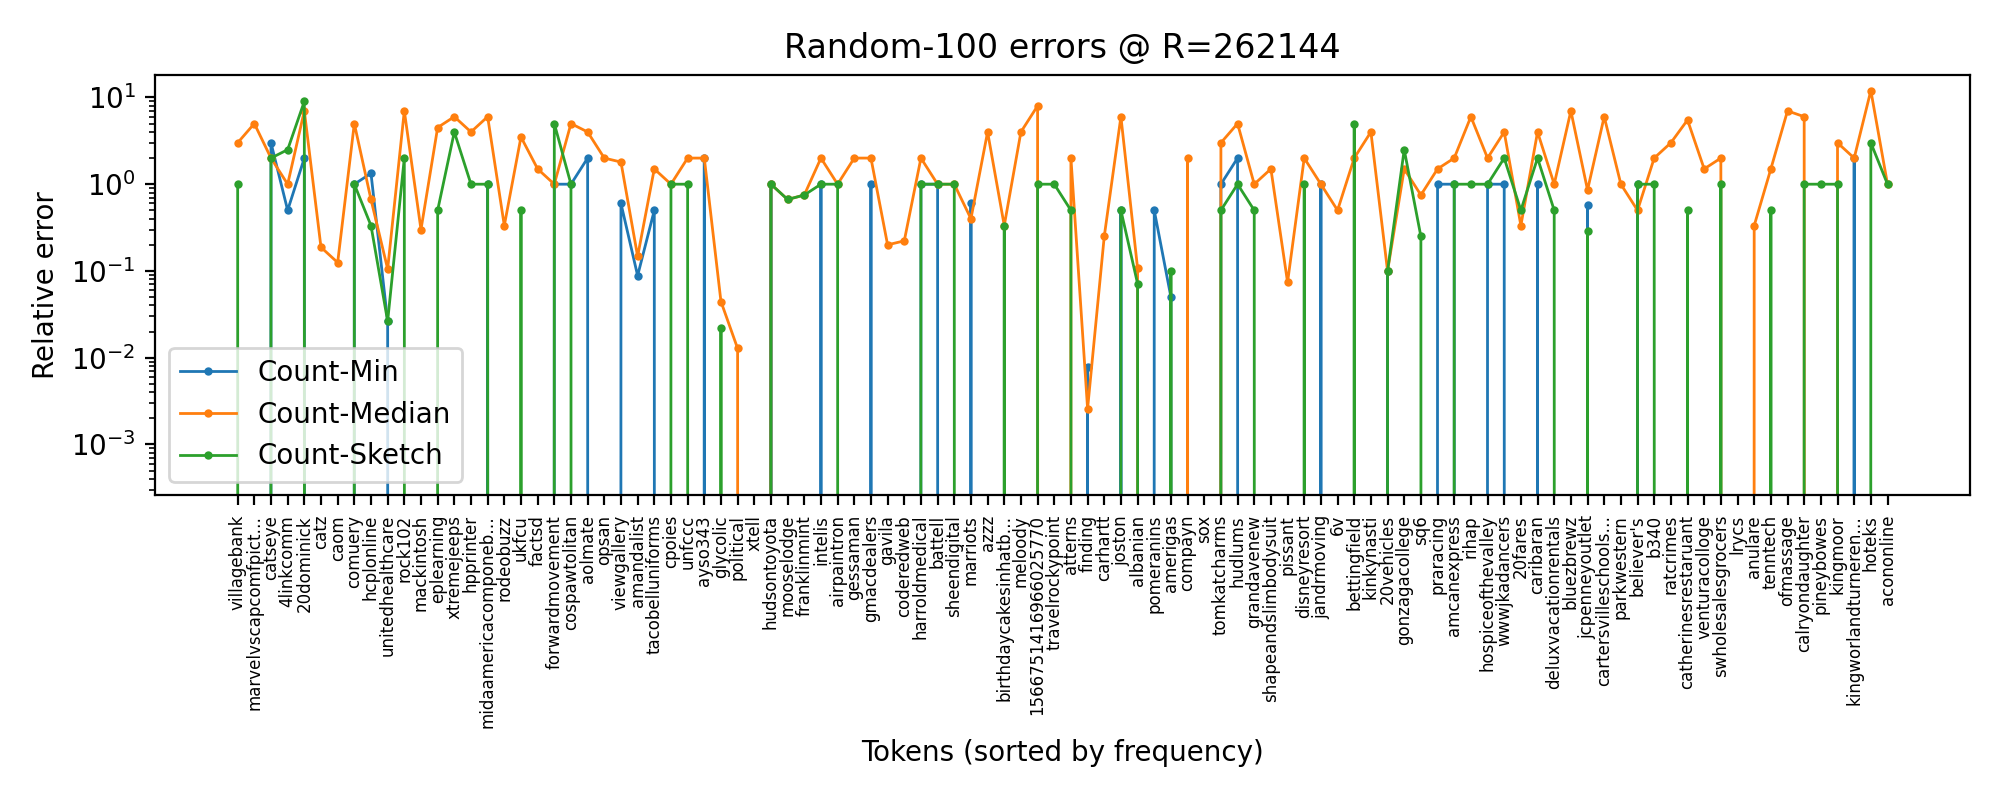
\includegraphics[width=\linewidth]{../outputs/a2/errors_R262144_Random_100.png}
    \caption{Random-100}
  \end{subfigure}
  \hfill
  \begin{subfigure}[t]{0.32\linewidth}
    \centering
    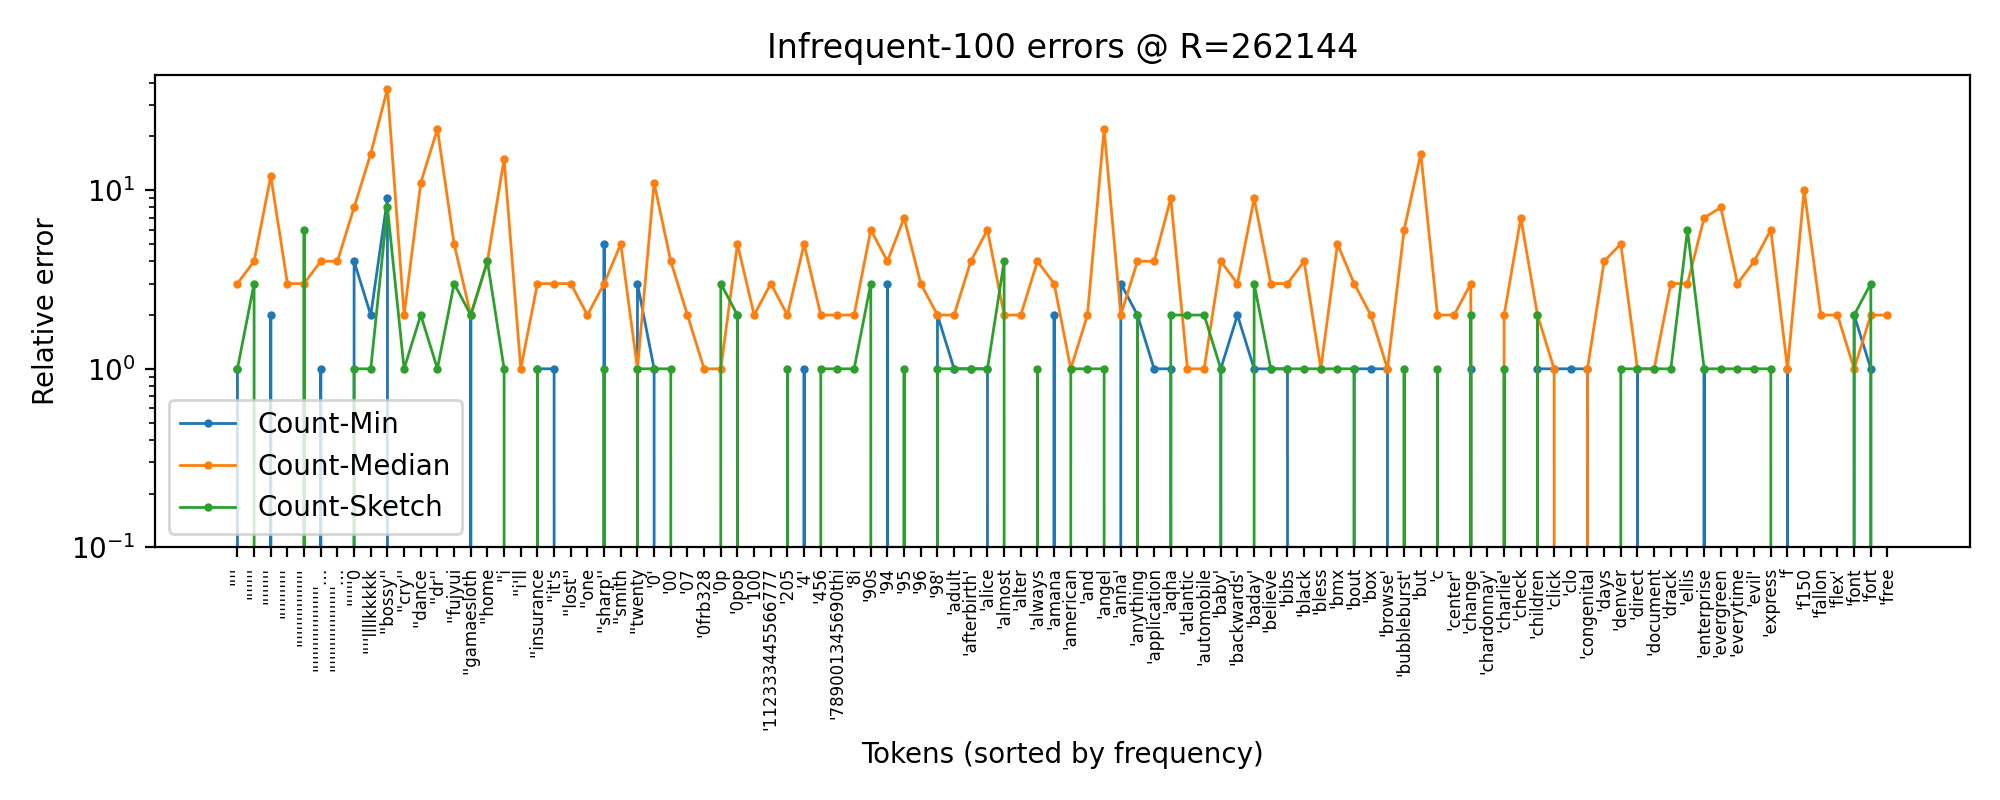
\includegraphics[width=\linewidth]{../outputs/a2/errors_R262144_Infrequent_100.png}
    \caption{Infrequent-100}
  \end{subfigure}
  \caption{Relative-error curves for $R=2^{18}$.}
  \label{fig:error-r262144}
\end{figure}

\begin{figure}[H]
  \centering
  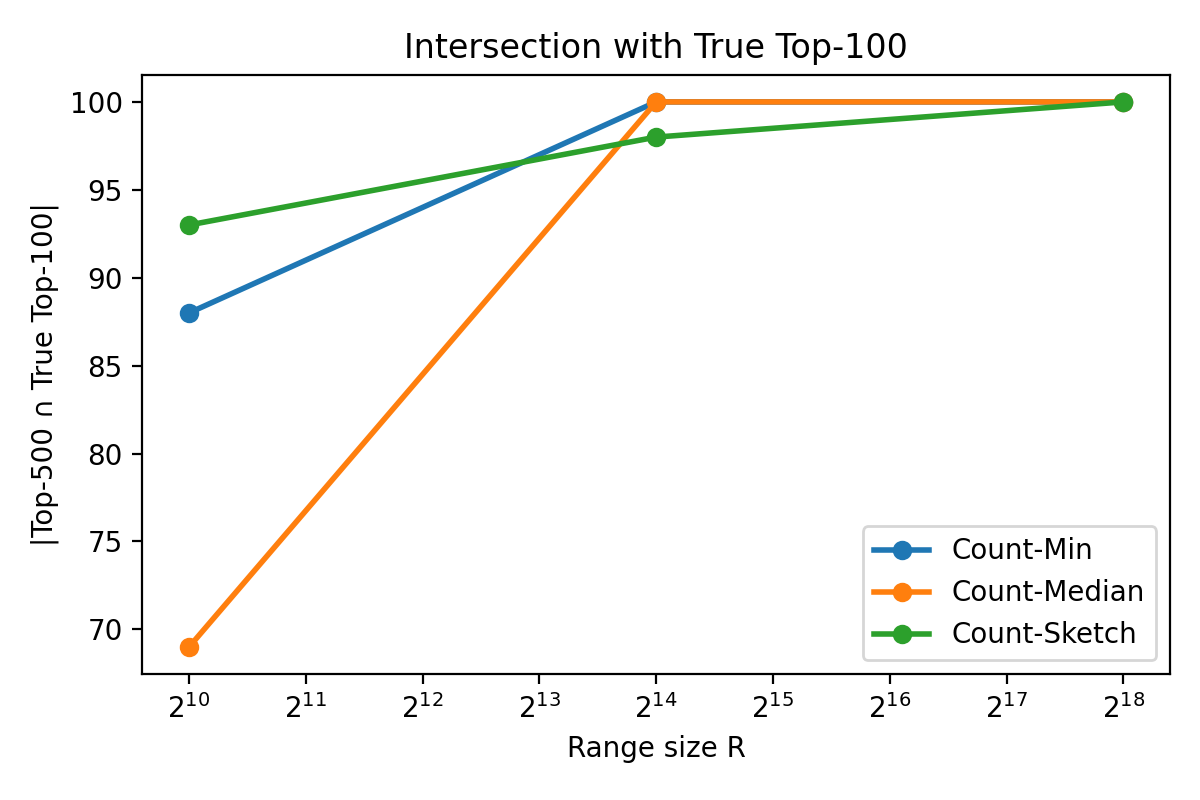
\includegraphics[width=0.55\linewidth]{../outputs/a2/top500_intersection.png}
  \caption{Intersection size of sketch top-500 with true top-100 across $R$.}
  \label{fig:top500}
\end{figure}

\section{Top-500 Intersection}
The heap-based tracker yields the set intersection sizes summarised in Table~\ref{tab:intersection}. Small values of $R$ drop many true heavy hitters, while widening to $R=2^{14}$ markedly improves overlap for every sketch in this sample.

\begin{table}[H]
  \centering
  \caption{Size of $\text{Top-500}_{\text{sketch}} \cap \text{Top-100}_{\text{truth}}$ (auto-generated from \texttt{outputs/a2/summary.json}).}
  \label{tab:intersection}
  \begin{tabular}{lccc}
\toprule
Sketch & $R=2^{10}$ & $R=2^{14}$ & $R=2^{18}$ \\
\midrule
Count-Min & 88 & 100 & 100 \\
Count-Median & 69 & 100 & 100 \\
Count-Sketch & 93 & 98 & 100 \\
\bottomrule
\end{tabular}
\end{table}

\section{Reproducibility Checklist}
\begin{itemize}
  \item \textbf{Generate outputs}: \verb|python main_a2.py --output outputs/a2|\ (optionally set \texttt{--limit} during testing).
  \item \textbf{Artifacts}: Plots land in \texttt{outputs/a2/} with filenames \texttt{errors\_R\{R\}\_\{category\}.png} and \texttt{top500\_intersection.png}; metrics appear in \texttt{outputs/a2/summary.json}. Each run also writes \texttt{error\_table.tex} and \texttt{intersection\_table.tex} so the report tables stay in sync with the most recent metrics-no manual edits required.
  \item \textbf{Dependencies}: Only the Python standard library plus \texttt{matplotlib} are required; a headless backend (\texttt{Agg}) is selected automatically.
  \item \textbf{Report build}: Run \verb|pdflatex tex/comp580_a2.tex| after generating plots to embed the figures.
\end{itemize}

\section{Conclusions}
The combined pipeline satisfies all deliverables: it streams the AOL log once, maintains exact frequencies for evaluation, compares three sketches at multiple width settings, quantifies relative errors for representative token buckets, and evaluates top-k recovery. The Count-Min sketch offers deterministic upper bounds but requires larger widths to suppress overestimation on sparse items, Count-Median provides unbiased point estimates at the cost of higher variance (especially with small $R$), and Count-Sketch trades reduced bias for manageable variance through signed updates. The logging instrumentation in \texttt{main\_a2.py} offers visibility into long-running jobs, making it practical to monitor the full-data execution required for the final submission.

\end{document}
